

\chapter{Discussion}\label{ch:discussion}

\subsection{Summary and key insights}

This thesis has introduced a two wave imaging technique 
- designed to generate and then immediately image a bubble -
and developed it from its theoretical foundation through to experiment.
The key themes are:
\nlist{
  \item The nucleation of the oil droplet into a bubble (\chapref{nucleation}).
  \item The response of the bubble contrast agent to an acoustic wave as {\em measured by ultrasound} (\chapref{measurement}). % as measured by ultrasound,  correct even for large bubble wall velocities.
  \item The response of a bubble to the two acoustic waves, the cavitation (driving) wave and the imaging wave (\chapref{mechanisms}).
}

The acoustic nucleation of a bubble was discussed in \chapref{nucleation}.
Here the capillary approximation was used to test the applicability of the technique.
It was found that type I nucleation, 
even of low boiling point chemicals such as the perfluorocarbons,
was likely to be beyond the capabilities of diagnostic ultrasound.
Not wanted to diverge from the technological norms of diagnostic imaging 
prompted the consideration of type III nucleation of water in our experimental chapters.

The validity of the capillary approximation was also considered in \chapref{nucleation}.
It was found to fall short in the case of the perfluorocarbons, 
where the distance over which vapour becomes medium is a significant fraction of the bubble's critical radius.
Calculating this density profile demonstrated that a density functional approach would have much to offer
the theoretical understanding of the acoustic nucleation of perfluorocarbon bubbles.
In particular, 
the high solubility of the perfluorocarbons to gasses such as carbon dioxide suggest that a 
study of the nucleation of these gases would be fruitful future work.


The low frequency wave that is used to initiate bubble formation will also influence the response of the bubble to a higher frequency imaging pulse.
It does so, 
as was determined in \chapref{mechanisms},
by altering the size of the bubble so that it is either closer or further from its resonance frequency.
This of course, 
has implications for bubble imaging when the bubble is long standing and is generated by other means.
One such application would be high frequency contrast imaging for small animals.
\Chapref{mechanisms} also introduced a two pulse technique to remove ambiguities
in the echo location of bubbles that can exist when using two acoustic waves.

Finally, \chapref{rationale} and \chapref{water_cavitation} presented the 
design  and then results of the two wave imaging technique of \chapref{mechanisms}.
The results, if not conclusive, are certainly suggestive of the techniques success
and warrant a further study and refinement.
Ambiguities regarding the bubble population would need to be resolved to move forward experimentally.


By far the most significant achievement of this thesis is found in \chapref{acousticSR}.
Ultrasound physicists have since the very beginning of their subject propagated the curious
error of defining their spatial and temporal coordinates with light.
When sound is use, 
as it should be for an acoustic measurement technology,
one finds that acoustics is a relativistic subject where the speed of sound has a privileged role.
It follows that ultrasound cannot measure a bubble wall collapsing at faster than the speed of sound,
and in \chapref{measurement} a new bubble model that has this property is derived.
Further, an exact correspondence between acoustics and electromagnetism exists.
As a direct consequence of this result it follows that 
\nlist{
  \item sound is a transverse wave of vorticity and Coriolis acceleration,
  \item sound has helicity - which corresponds to the hydrodynamic helicity.  
    Sound has integer spin.
  \item The exists an acoustic current that is conserved.
  \item The acoustic current obeys an acoustic analogue to the Lorentz force law.
}
The importance of these observations should not be underestimated.

Given the existence of an {\em acoustic spin},  and a conserved {\em acoustic charge},
that obeys an {\em acoustic Lorentz force law},
it does not seem to far fetched to ask whether there exists an {\em acoustic electron}.
Such an idea, of course, 
revives the very old theories of Bjerkness\cite{Bjerknes1905}, Maxwell\cite{Maxwell1861} and Thomson\cite{Thomson1931}.
All that we say on the matter is to note that 
Hick's spherical vortex, the favoured model of many in the nineteenth century,
has a conserved angular momentum\cite{Pekeris1976,Pekeris1977} and a conserved spin\cite{Moffatt1969,Moffatt1988}
when measured acoustically.

Finally, 
we have shown that there is nothing intrinsically special to light.
The significance of the speed of light results from its  role in the measurement process.
%If sound is used in place of light for measurement, then the speed of sound is equally important.
It is privileged if we believe only what we see.
There is much to understand in the world if we are prepared to be more open minded.


% that distance over which dThe capillary approximation was used 
%In \chapref{nucleation} the suitability of perfluorobutane and perfloropentane  for the oil droplet
%as oil droplets capable of being vapourised by diagnostic ultrasound pulses 
%was investigated.
%The nucleation rate was calculated with the classical equation and its failure to predict experiments was explained by the  density functional approach.
%The explanation was entirely in keeping with the investigations of \cite{Oxtoby1988} and co-workers.

%A semi-empirical density functional approach was used to fit a Lennard-Jones 6-12 potential to empirical bulk vapour pressure
%and density data. %, and surface tension taken from the literature - the three bulk properties of the classical theory.
%The nucleation rate as a function of pressure was then obtained,
%%with a pressure of  ... required to nucleate for perfluorobutane and a 
%with a pressure of ... required for perfuoropentane.
%This compared with the value of  ... that was calculated with the classical theory.
%Since the inaccurate capillary approximation was {\em not} used in this calculation, 
%there is hope for its accuracy.

%The  response of a bubble as  {\em  measured by ultrasound} was then modelled. %how the oscillations of the bubbles manifest themselves when measured acoustically.
%To do so the discussion was broadened somewhat to acoustic measurement in general.
%It was noted that ultrasound defines the temporal and spatial locations of entities within its world view from the time of flight.
%An {\em a priori} sound speed is  used to convert these times into distances.
%If  invariance to  inertial motions  holds (as it does in all known physical theories) 
%then it was found that the acoustic pulse-echo definition of time and space becomes identical to the 
%standard radar definition that uses light.
%This means that ultrasound is a relativistic theory where the sound speed takes the role of the speed of light.


%The physical reason for this are clear.
%It is impossible to measure, by pulse echo, an entity that moves away from the transducer at speeds that are faster than the speed of sound.
%The sound will never catch up with the entity, and  there will never be an echo.
%The sound speed therefore sets a limiting velocity to what can be measured,
%and the spatio-temporal locations that are assigned by the pulse-echo technique become warped as this speed is approached.
%To describe the world as it is measured acoustically the transformations induced by the pulse-echo technique must be included in the formalism.
%This is precisely what the Lorentz transformation, the $\gamma$ factor, does.

%A theory that predicts the outcome of acoustic measurements must therefore be Lorentz invariant.
%Otherwise, the notion of time and space used in the theory is not consistent with the pulse echo technique actually used.
%A Lorentz invariant version of the Keller-Miksis equation was derived in \chapref{measurement}.
%To do so a Lorentz invariant description of an ideal fluid was required.
%Such a description already exists in the relativity literature.
%It was applied  immediately by simply equating the speed of sound with the speed of light.
%The result is a description of the bubble that describes the locations of the bubble wall as measured with ultrasound.

%The acoustically-measured-Keller-Miksis equation was then employed to 
%predict the measurements of the contrast agent when two acoustic waves are present.
%We only considered the case of interest in this project, 
%a low frequency driving wave and a high frequency imaging wave.
%It was found that the driving wave manipulates the bubble by altering its size.
%The resulting scatter of the imaging wave is increased or not depending on whether the bubble 
%is pushed towards or away from resonance by the driving wave.

%This is of particular interest as it suggests that the two wave technique can be applied more generally
%to manipulate the bubble.
%To image at a higher frequency the imaging wave can be timed to coincide with the bubble when it is being compressed by the driving wave.

%The excess scatter over a large phase space of frequencies and amplitudes was explored.
%Even though the response of the bubble to the driving wave 
%is in general nonlinear - the general phase dependence of the imaging wave upon the driving wave was found to be remarkably resilient.
%The parameter space was sampled by a monte carlo technique to find the set of parameters that maximise the scattering of the imaging wave.
%The results are given in \tabref{MonteCarloResults:short}.
%%A two pulse technique was introduced to evaluate the excess pressure generated by an imaging wave.
%%The purpose of this was to eliminate the bubble's response to the driving wave
%%that was picked up by the imaging transducer.
%%When simulated, temporal ordering was thereby reintroduced to the imaging wave.


%Interestingly, when the formulae of acoustics are derived for a fluid as measured by pulse echo,
%the resulting wave equation is identical to Maxwell's relation of electromagnetism.
%This  result was explored  in \chapref{interactions},
%where the  correspondence between the two theories is identified.
%The equivalence of the theory of light, when space and time are defined optically,
%with the theory of sound, when space and time are defined acoustically, 
%is highly suggestive.
%Could it be that relativity is nothing more than a manifestation of the choice of propagating signal?
%If so, then who is to say that a `better' signal does not exist?






% These properties have  encouraged other groups,
% independently of our own, 
% to investigate the potential of using ultrasound to generate a bubble from  perfluoropentne droplets. 
% %This distinguishes the investigation here from many  other groups.
% \todo{cite Burns and Rappaport here, comment on short pulses of  Miller2000\cite{Miller2000} (Kripfgans)}

% \todo{bubble encapsulation Pisani2006\cite{Pisani2006}}



% \todo{Evaporation velocity is about 14.3 metres per second in HongChul2005 but citing shepherd and sturtevant 1982.}


%\section{Future work}


%The density functional investigation of \chapref{nucleation} can be used to calculate the nucleation rate 
%without having to make the capillary approximation\cite{Oxtoby1988}.
%Furthermore, it can be readily extended to a binary fluid\cite{Talanquer1994, Talanquer2001}.
%This is what ultimately needs to be done.
%It is important to get a theoretical feel of how nucleation is affected by mixing the perfluorocarbons.
%It would also be interesting to investigate whether it is the perfluorocarbon itself that causes the nucleation event.
%Another possibility is that it role of  perfluorocarbon is to act as a highly soluble medium for much more volatile gases.
%%It is difficl are difficult to realise experimentally
%
%In \chapref{measurement} scattering cross section simulations were presented
%and it was claimed that the acoustically measured theory was correct even to high speeds.
%This provides a direct experimental test to the theory of \chapref{measurement} - 
%one that should certainly be pursued.
%
%The dependence of the bubble's high frequency scatter on the phase of an  driving wave, found in \chapref{mechanisms},
%has applications to conventional bubble imaging.
%As noted in the text, 
%the results of \chapref{mechanisms} imply that it should be possible to manipulate a bubble scatter by using a second, lower frequency wave.
%This could be used, for example, 
%to extend the frequency range of existing bubble technology.




% \subsection{Experimental Objectives}


% \subsection{Experimental Method}
% \begin{figure}[p]
%      \centering
%      \subfigure[The radius of the bubble is changed by the low
%      frequency wave.  This will alter the bubble's resonance frequency.]{
%           \label{fig:change_radius}
%           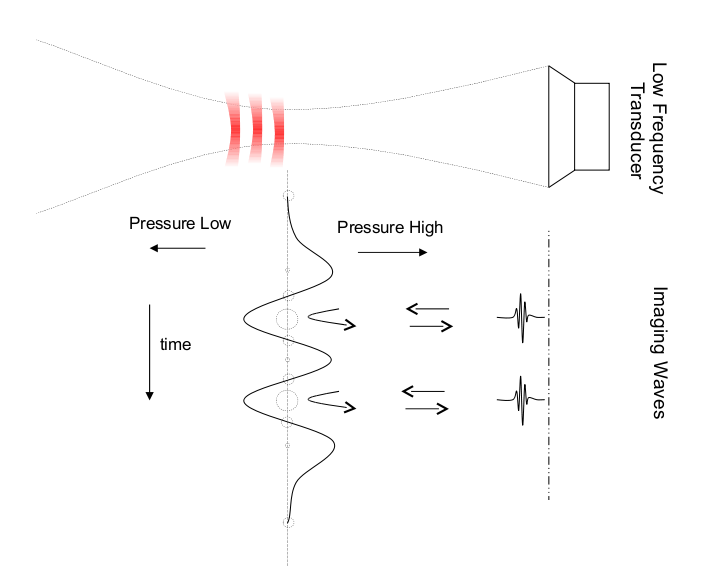
\includegraphics[width=0.8\textwidth]{change_radius.png}}
%      \hspace{1cm}
%      \subfigure[By timing a high frequency wave to meet the bubble
%      while it is under the influence of the low-frequency wave, the
%      bubble can be induced to resonate at higher than usual
%      frequencies. This is because the bubble will transiently be
%      smaller (when it is compressed) and because it will experience a
%      Doppler shifted imaging wave. ]{
%           \label{fig:both_waves}
%           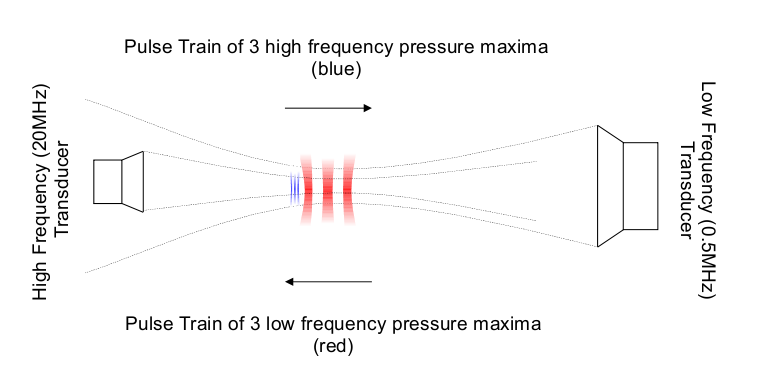
\includegraphics[width=0.8\textwidth]{both_waves.png}}
%      \caption{Low and high frequency pulses emitted.
%      }
%      \label{fig:general_idea}
% \end{figure}


% The two transducers need to overlap at a common focus and we wish to
% interrogate all phase relationships between the two waves.
% This is most easily achieved by having the two transducer's facing
% each other,
% as drawn in \figref{arrangement}.
% In this arrangement the firing of the two pulses is co-ordinated so that the waves meet at
% their common focus at the same time.
% As they pass through each other at twice the speed of sound the two waves will pass through all
% possible phases.
% When imaged by the high-frequency wave the phase of the low frequency
% wave will manifest itself as a
% function of depth.

% The limited bandwidth of the high-frequency transducer is relied upon
% to filter out the direct transmit of the low-frequency wave.



% \begin{figure}[h]
%      \centering
%           \label{fig:arrangement}
%           \includegraphics[width=0.4\textwidth]{arrangement02.1}
%      \caption{The arrangement of the two transducers.  From the first
%        year, the high frequency transducer has been replaced with the
%        cortex scanner, a commercial skin scanner containing 20MHz scanning single element transducer. }
% \end{figure}
% %The two ultrasonic beams need to overlap at a common focus as
% %illustrated in \figref{both_waves}.
% experiments has now been  replaced by a scanning single element 20MHz
% transducer that is a part of a skin scanner manufactured by Cortex
% technology (Haadsund, Denmark).

% With the Cortex we have  access to the frame trigger output, the
% A-line trigger output , the
% direction of the scan of the transducer and the RF data.
% It has a slow frame rate of  approximately 3-4Hz.
% The cortex has a curious although very useful pulse sequence, with two
% A-line-pulses in rapid (100 microsecond) succession, followed by a large (millisecond
% scale) interval.
% This is illustrated in \figref{cortex_gate}.

% \begin{figure}[h]
%      \centering
%           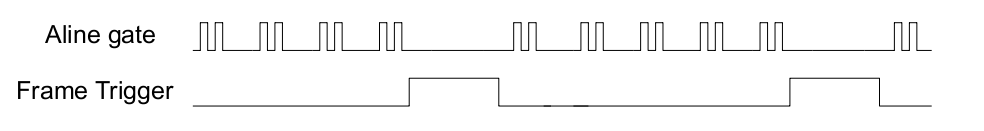
\includegraphics[width=0.8\textwidth]{cortex_gate.png}
%      \caption{The cortex fires two A-lines in quick succession before
%        repeating the sequence after a
%      relatively large pause.}
%           \label{fig:cortex_gate}
% \end{figure}


% The focal length of the low frequency transducer is longer than that
% of the Cortex
% transducer
% and as such it needs to be triggered before the cortex in order for
% both signals to reach the sample at the same time.
% It is therefore impossible to time the low frequency transducer to
% propagate through to the sample  at the same time as the low
% frequency pulse.
% The two pulses from the cortex enables this problem to be overcome,
% however.
% The first pulse of the cortex A-line doublet is used to trigger the low
% frequency transducer so that the first low frequency pulse arrives at the
% sample at the same time as the second high frequency pulse.
% In this way we generate two interleaved images, with adjacent A-lines
% imaged with the pulse off, and then the pulse on, etc.
% The second low frequency pulse  (triggered from the second
% A-line doublet) is ignored.

% \subsection{Incident Waves}

% \section{
% Part I: Nucleation Study
% }
% A characteristic of the experiments of this project are that they are
% rapid to carry out,
% but are very laborious to calibrate.
% As an example,
% the signal driving  the low-frequency wave can be attenuated with the
% flick of the switch, 
% but to determine the corresponding pressure field requires a lengthy
% beam plot.
% For this reason the results presented here have a `look and see' feel
% about them.
% The results have not reached a stability for which their extensive
% calibration is worthwhile.

% The main experimental parameters that are 
% subject to our control are:
% \nlist{
%   \item
%     The relative phase between the low-frequency and imaging wave.
%   \item
%     The pressures of the two waves.
%   \item
%     The frequencies of the two waves.
%   \item
%     The pulse-length of the two waves.
%   \item
%     The (droplet) size of the (emulsion)/bubble.
% }
% The first of these is well sampled by  virtue of the experimental
% setup.
% The two waves pass through each-other and so in {\em every} image {\em
%   all}
% phases between the two waves will be sampled.

% Sampling the pressure of the low-frequency wave is also
% straight-forward.
% A wide range of driving pulses are chosen to vary the peak pressure
% at the focus.
% In addition, since an 2D image is formed, 
% the spatially varying pressure field of the low frequency wave 
% will be imaged in  {\em every } image.
% The pressure of the imaging wave is much harder to control,
% for it is controlled internally by the scanner.
% %Indeed, it would be helpful to turn the imaging wave off altogether.
% %This cannot be achieved without modifying the scanner, however.
% The pressure ranges experimented with range from 0 through to $>1$ MPa
% peak-negative.

% Likewise, by choosing different  transducer, a range of
% frequencies  can be used for the two waves.
% Although our choice is not completely free.
% The high frequency pulse ideally should last for only a small fraction
% of the period of the low frequency wave.
% In addition, 
% when the difference in frequency between the low and high frequency transducers
% becomes small the direct transmission of sound between the transducer's
% becomes a problem for the anti-parallel setup of the transducers.
% Imaging frequencies of between 7.5 and 20 MHz have been tried, 
% along with low-frequency waves of between 0.5 and 2 MHz.
% The results presented here were used a 0.5 MHz low frequency wave and
% a 20 MHz imaging wave, unless otherwise stated.

% The pulse length of the imaging wave should be short, 
% although when imaging is achieved with a scanner, such as the cortex,
% then this parameter cannot be changed.
% The pulse length of the low frequency transducer is readily set.
% To avoid bubbles growing (by rectified diffusion), fusing (by Bjerknes
% forces) and collapsing (by instabilities in the oscillations) the low-frequency
% pulse should also be short.
% However, to reduce forward transmission the  frequency output of the
% low frequency wave should not be 
% too broad-band.
% 10 cycles is used in these experiments.

% The size of the bubbles/droplets is not simple to control.
% In general a fairly broad-range of sizes is present, even for the
% commercial agents,
% although one of the advantages of using commercially available
% contrast agents are that their size have been well studied.
% It is not possible to directly size the bubbles formed in cavitation,
% even though this is of interest.
% This is because the bubbles are too short lived.
% Finally, 
% sizing the perfluoropentane emulsion is also hard.
% This is because perfluoropentane is a transparent fluid with
% essentially the same refractive index as water,
% and so optical sizing becomes hard.
% The best that can be done so far is to bound the size distributions by
% passing the emulsion though a filter.
% For other reasons it is desirable to attach a fluorescent
% marker to the emulsion, but as a bonus this should help size the
% droplets.




% \subsection{Commercial Microbubbles}\label{sec:bubble_exp}

% \begin{figure}[h]
%      \centering
%   \subfigure[B-mode image of Levovist without the presence of the
%   low-frequency wave]{
%           \label{fig:levovist_without}
%           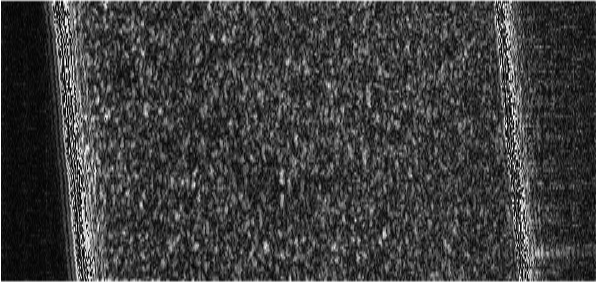
\includegraphics[width=0.8\textwidth]{cortex_without.png}}
%      \hspace{1cm}
%      \subfigure[B-mode image of Levovist with the presence of the
%   low-frequency wave]{
%           \label{fig:levovist_with}
%           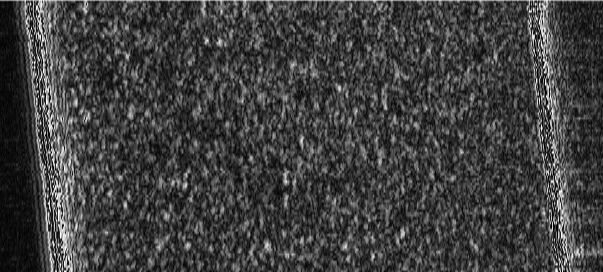
\includegraphics[width=0.8\textwidth]{cortex_with.png}}
%      \caption{Cortex B-mode images of Levovist with and without the low
%        frequency wave. 
%        The cortex operates at 20MHz and the low frequency wave is at
%        0.5MHz.
%        The low frequency transducer has a peak-negative pressure of
%        about 0.2 MPa.
%        The scanner is to the left of the image and
%        the heavy parallel signals are the from the sample holder, an opticell.
%      }
%      \label{fig:bubble_data}
% \end{figure}


% So far the experimental work to detect an effect of the low frequency
% wave has not been successful.
% \Figref{bubble_data} is typical, with no discernible difference
% between when the pulse is on to when it is off.


% There are a number of possible reasons for this.
% Firstly, is the possibility that 20MHz is too high a frequency (too far from
% resonance)
% for the changes in bubble size to be detectable.
% Lower frequencies were tried (down to 7MHz) with the same result
% although the full parameter space was not so thoroughly   investigated
% as for the 20MHz imaging wave.
% %The bubble simply does not get sufficiently small even when the low
% %frequency wave is present to make the change evident.
% %The main method for a signal to be detected at this frequency is via
% %the Doppler aspect of our experiment. 
% %However, the Doppler method for signal detection is relatively new to
% %our thinking and our data has not yet been analysed in its light.

% Further possible problems could be associated with our geometry.
% In having two opposing waves we are attempting to detect a change in
% scattering cross-section with distance through the sample.
% This method should work well with a mono-disperse distribution of
% bubbles.
% However, there is in fact quite a broad distribution of bubbles.
% It is possible for the effect to be present without it being
% observed if through the sample we are increasing the scattering cross
% section uniformly, because we eliciting a response from bubbles of
% different sizes at different positions from within the sample.
% Having a parallel beam solution would overcome this.
% For the parallel arrangement it could be possible for the two waves to
% simply propagate until they come 
% across a bubble of the correct size for the now arbitrary phase
% relationship chosen between the two waves.

% Additionally, for the banding anticipated to be observed
%  the  bubbles need to oscillate with the same
% phase with respect to the low frequency wave.
% This will not occur as the phase relation between the bubble wall and
% the insonating pulse is a function of the bubble size (and therefore
% the resonance frequency).
% The distribution of bubble-sizes currently possible in bubble physics is
% rather wide.
% This requires that the low frequency is chosen to be  away from the resonances of
% the bubble, which means that the radial oscillations (and therefore the
% effect) are small.
% The need for spherical oscillations imposes similar problems.
% Further, bubbles smaller than resonance size will tend to move towards pressure maxima,
% coalesce   until they are larger than resonance and then  move
% away.
% Finally, it is important to avoid a partial `standing' waves within
% the sample holder.
% This is harder than it may seem, as seen for the 30 cycle low frequency wave
% in \figref{standing}


% \begin{figure}[h]
%      \centering
%           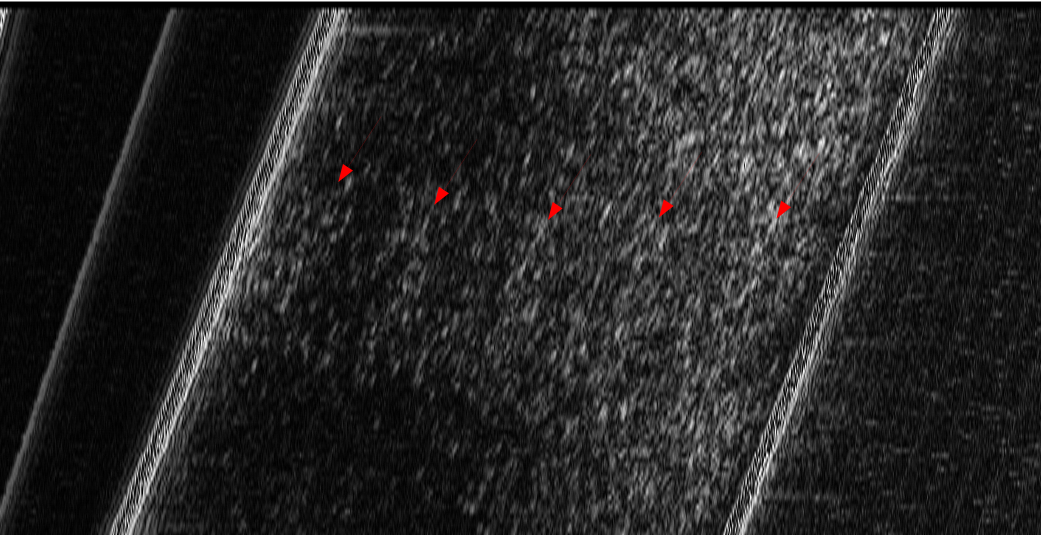
\includegraphics[width=0.8\textwidth]{streaming.png}
%      \caption{A 30 cycle $\half$ MHz wave generated a `standing wave'
%        pattern of nodes/anti-nodes within the sample holder, as seen
%        with the red arrows  The bubbles have been streamed in the
%        region of the focus (the middle of the image) from the bottom
%        of the sample holder (the right of the image) to the top.
%        Away from the focus there are no bubbles at the top of the
%        sample holder (the dark regions on the bottom left and top left
%        of the image).}
%           \label{fig:standing}
% \end{figure}

% To evaluate whether any effect has been caused by the low frequency
% wave also has its problems.
% The images are not very stable, the bubbles float, their densities
% change to match any kind of standing wave and they coalesce.  It
% makes the results from averages across frames not-entirely conclusive.

% In addition, the imaging technique is difficult to distinguish from harmonic imaging.
% How can we be sure that any observed influence of the low frequency
% wave is not simply due to the forward transmission of harmonics of the
% low frequency wave, rather than a change in acoustic backscatter of the
% bubble to the imaging wave?

% In short, a better understanding is required in order to narrow the
% parameter search.
% This can be achieved with the computational study already discussed.


% A method is needed to statistically asses the images.
% One way to do this is to produce a pressure map of the low
% frequency transducer as seen by the high frequency pulses when they
% are reflected by bubbles.
% This can then be overlayed onto images to get the `ambient' pressure seen at each location.
% A scatter plot of intensity vs pressure is then drawn,
% which can then be compared to a Rayleigh distributed for scatter to
% infer the mean.
% If this line is not horizontal the imaging technique has worked,
% otherwise it has not.
% %Whether time is devoted to actually 


% \subsection{Cavitated Water}\label{sec:water_vapourisation}



% \begin{figure}[h]
%      \centering
%           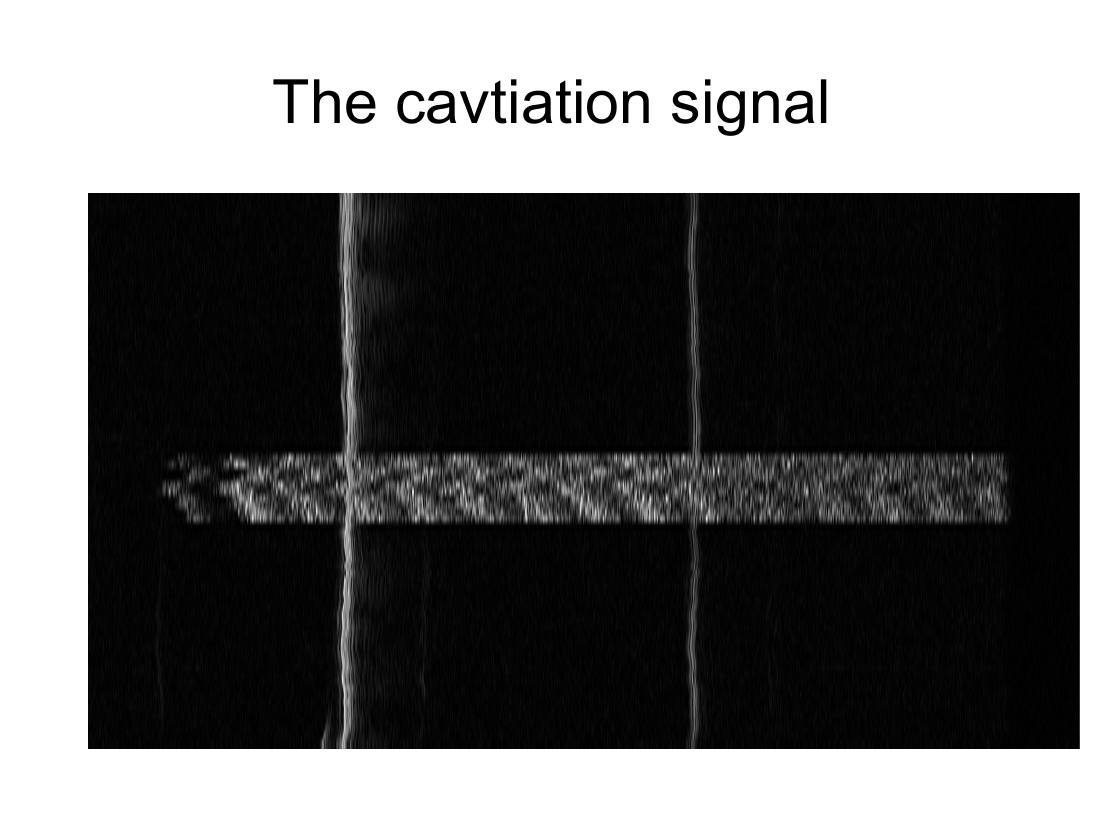
\includegraphics[width=0.8\textwidth]{emulsion_cavitation_signal.png}
%      \caption{Typical cavitation signal seen in bubbly water.
%      The two long vertical lines are the reflections of the sample
%      holder.
%      The imaging transducer is to the left,
%      the low-frequency transducer is to the right.}
%    \label{fig:cavitation}
% \end{figure}

% Before attempts were made to cavitate a perfluoropentane emulsion,
% water was  cavitated to give indication as to the type of images that
% were to be expected.
% These could then be compared with the oil-drop emulsion.

% In \figref{cavitation} the low frequency wave has been fired for the
% middle 10 A-lines of bubbly (tap) water.
% In this experiment 10 cycles of a 2 MHz wave were used as the low-frequency
% wave.
% The pressure was high, with a peak negative pressure of over 1MPa.

% There was some jitter in the firing of the low-frequency waves in this
% experiment introduced by a signal conditioner necessary for an FPGA
%  used to count the A-lines.  This is the most likely explanation
% for the vertically wavy appearance.

% Nevertheless the signals are interesting for a number of reasons.
% Of particular interest is the (horizontal) banding seen in the images that matches the
% wavelength of the low frequency transducer.
% While the sizes of the bubbles generated in the \figref{cavitation}
% are not known,
% they are expected to be small and  $0.1$ micron seems the correct
% order.
% It is therefore tempting to compare the banding structure seen in the
% normalised scattering cross-section seen computationally in
% \figref{xs}.
% This is, of course only one possible explanation for the banding
% structure in \figref{cavitation},
% although it seems at least as good an explanation as any other that
% can be put forward.





% \subsection{Emulsion}\label{sec:emulsion_exp}

% \begin{figure}[h]
%      \centering
%           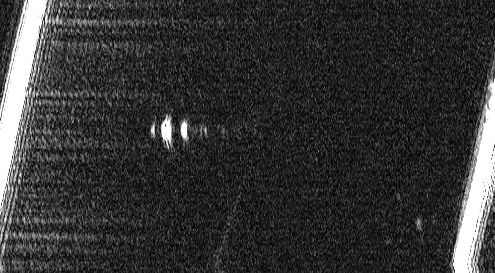
\includegraphics[width=0.8\textwidth]{emulsion_vaporisation.png}
%      \caption{When the low-frequency wave is on it is possible to
%        suddenly generate these bright signals.  These persist even
%        when the low-frequency wave (40 cycles at 2 MHz) is turned off.
%        The bright regions are fairly
%        buoyant, in that when the low-frequency wave is off they neither
%        sink with the density of the perfluoropentane, nor rush to the
%        surface of the sample holder as a large gas-bubble would with
%        gravity.
%        This suggests that they a mixture
%    of fluid and gas.}
%           \label{fig:vaporisation}
% \end{figure}

% The emulsions are made by sonicating perfluoropentane in degassed
% water.
% In the first experiments the emulsifier lecithin was also included,
% although more-recently it has been found to be unnecessary.
% Surprisingly stable emulsions form even without the emulsifier.

% This was good news as the lecithin proved problematic.
% Firstly the degree to which lecithin was stabilising the emulsion and the
% degree to which it was forming micelles without any emulsion was not
% possible to explain.  These micelles would be a confounding factor in
% our experiments as they would act as nucleation sites for cavitation
% irrespective of whether there was any emulsion present.

% In addition, the lecithin clogged up any filter through which we
% attempted to pass the emulsion, thus removing the opportunity to
% provide a bound on the size of the emulsion.


% The low frequency wave is able to induce a signal not seen without the
% emulsion and lecithin mixture.
% A typical example is seen in \figref{vaporisation}.
% These signals are large in size and seem neither to float nor
% sink too rapidly.
% Again the band structure is evident but due to the near-neutral
% buoyancy 
% of the bright regions this banding could easily be down to the partial standing
% wave that formed similar banding in \figref{standing}.

% Without the lecithin the experiment is much improved.
% The now just perfluoropentane and degassed water emulsion passes very
% easily through a 200nm syringe filter when injected into the sample
% holder.
% Not only can signals similar to \figref{cavitation} be formed at lower
% pressures than for degassed water, 
% highly transient but bright signals of a different signature are seen
% at the focus of the low frequency wave.


% \begin{figure}[h]
%      \centering
%           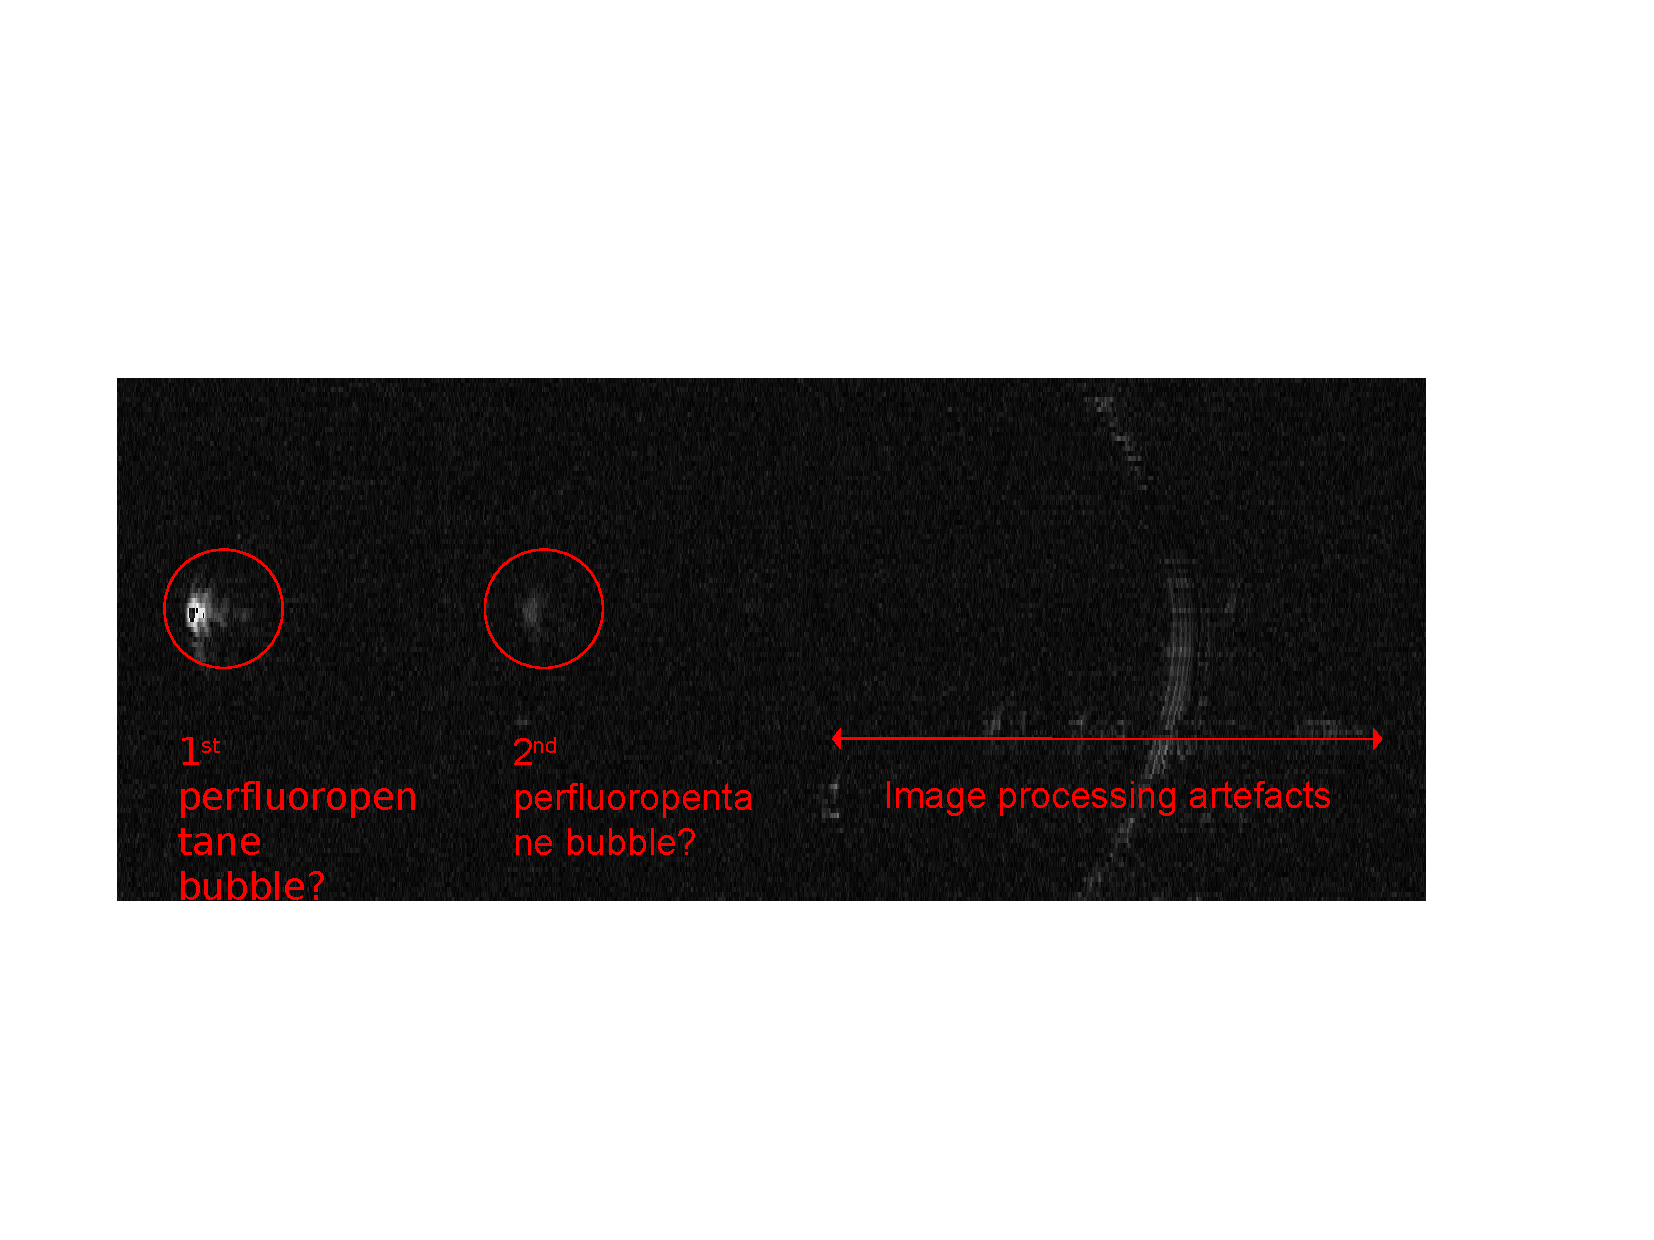
\includegraphics[width=1.0\textwidth]{vapour.pdf}
%      \caption{
%        A subtraction image.
%        The signal returned to the imaging transducer when the
%        low-frequency wave is off is subtracted from when it is on.
%        The low frequency wave is at 0.5 MHz for 3-4 cycles (including
%        those generated by transducer reverberation.  That is the peak
%        pressure off each maxima is not the same.
%      }
%      \label{fig:vapour}
% \end{figure}

% In \figref{vapour} such as signal is plotted.
% The image is formed by subtracting alternate A-lines.
% For each alternate A-line, one is imaged with the low frequency wave
% off, and one is imaged with the low frequency wave on.
% The bright signals that remain, therefore,
% are short-lived, appearing and vanishing with millisecond lifetime 
% between alternate A-lines.
% The signals shown in \figref{vapour} remain at the same location for
% many consecutive frames.

% Since there is nothing other than oil and water \figref{vapour}, and
% because the water does not produce such images at these pressures,
% confidence can be taken in interpreting the signal as a perfluoropentane
% bubble.  
% This has not been confirmed by other means, however.

% Finally we note that signals similar to \figref{cavitation} can be
% made with the oil emulsion.
% However, the cavitation events are much more violent at lower pressures than for degassed water.
% This is known since the cavitation events can be heard audibly to a
% much greater extent for the emulsion.
% An audio-frequency cavitation detector would help quantify these observations.



% \subsection{Water}

% \subsection{Emulsion}



%%% Local Variables: 
%%% mode: latex
%%% TeX-master: "tshorrock_thesis"
%%% End: 

% LocalWords:  Lennard perfluorobutane perfuoropentane
